\documentclass[authoryearcitations]{UoYCSproject}
\author{James White}
\title{Embedding and Visualising the Internet}
\date{\today}
\supervisor{Richard Wilson}
\wordcount{15527}
\CSAI
\abstract{
Most of us use the internet every day, but do we really understand what it looks like? There is a very predictable tiered structure to the internet which makes it difficult visualise adequately. This project will attempt to use the properties of non Euclidean space, namely hyperbolic space, to produce visualisations of the internet based on geographic data. It is hoped that these visualisations could be used to further understanding of the internet and its structure.
}

\acknowledgements{
I would like to thank my supervisor, Richard Wilson, for proposing this project and giving me the chance to work on something which has proven to be truly enjoyable and which has allowed me to learn so much.
}

\begin{document}
\maketitle

\cleardoublepage
\part{Preliminaries}
\label{sec:prelims}
\thispagestyle{empty}\cleardoublepage
\chapter{Introduction}
\label{cha:Intro}

Most of us use the internet every day, but do we really understand what it is? It was once described as being "a series of tubes", which, while incorrect, is not far from the truth. The internet itself is effectively a construct which has arisen through the \textit{inter}connection of smaller computer \textit{net}works and exists only as a whole because these networks required connections to others to communicate information. More and more networks required these connections and eventually it became possible to communicate with most other networks by forwarding information across many others. 

However, networks were often set up in places which did not offer another network for a connection and a more rigid way of connecting to the internet was required. Companies specialising in providing connection to the internet began appearing, these were the first Internet Service Providers (ISPs). An ISP offers an internet connection as a service, providing an access point through which to route data, or traffic, to the rest of the internet. There were of course very few ISPs when the internet first began, as the initial investment in laying the physical cables and equipment necessary was very large, many of these first ventures were government backed and publicly funded. 

When a business or person wishes to connect their network to the internet they must purchase the ability to do so from an ISP that operates in their area, sometimes they will have a choice, sometimes not. That ISP then must forward any traffic which that customer generates to the correct network on the internet; this is a \textit{provider-customer} relationship. But what if that ISP does not have a direct connection to this network? It is insufficient to simply fail to deliver the traffic, customers would not accept that! Instead it is the prerogative of the ISP to provide as complete traffic forwarding capabilities as possible. ISPs accomplish this through peer agreements with other ISPs, where each ISP agrees to forward the others traffic if it can. This is a \textit{peer-peer} relationship and is the reason for the widespread adoption of the internet as a communication medium. It is important to consider that ISPs must have as many peer agreements as they can, given their physical location, as this makes them more attractive prospects for new networks. 

\section{Internet Structure Background}

Considering how the internet is structured may seem like a difficult question at first, but the structure is actually very simple. If a small business wishes to connect themselves to the internet then they make an agreement with a local ISP in order to do so. This agreement is effectively the same one the ISP makes with all their customers, which may number from a few to millions. If we take an ISP with a million customers, for example, then they must connect to another ISP which allows them to forward all traffic generated by these customers to the correct network. However, as these peers also connect to peers, this reduces the number of peer-peer connections required to very low numbers, way below the number of provider-customer links. 

In truth, all ISPs do not always peer with others, instead there is a hierarchy of sorts through which \textit{lower-level} ISPs pay \textit{higher-level} ones to forward their traffic in the same way a business would a their ISP. These are still provider-customer relationships but they serve to link ISPs with others that are far away physically, through an intermediate ISP. This type of internetworking causes the internet to have a very predictable and interesting structure. 

ISPs which reside at the top of the hierarchy have connections to other large networks in order to provide long range transit for large amounts of traffic. Those in the middle tiers often sell links between higher tier ISPs and lower tier ones, but they will always have more customers than suppliers, meaning they will link many low-tier ISPs to a single high-tier one. Low-tier ISPs will often link many small networks to a single mid-tier network. At the very bottom tier a network will be connected to a single ISP. It is important to note that the internet does not have a rigid tier system, this is simply an emergent property of the way networks are interconnected.

If the internet were to be represented as a tree, then it would have an extremely high branch factor, which causes it to be very difficult to effectively visualise. Though, strictly speaking, the internet cannot be a tree because it has no defined root node and there is no concept of parent and child in a peer-peer link. However, the internet does have a very densely linked core, where few, high degree nodes are connected to others of the same kind. In addition, moving out of the core and down the \textit{tree} reveals many smaller nodes which only have a single, or very few, connections. Clearly, the further from the core a node is the more nodes exist \textit{near} it, in practice this is actually an exponential increase and it is very difficult to visualise graphs such as this due to there not being enough space for the low-tier systems to fit. This begs the question; is there a way of visualising the internet which preserves this hierarchical structure?

\section{Aims}
\label{sec:aims}

The aim of this project is to construct a graph of the internet and embed it into a space which supports its properties, namely a hyperbolic space. The project will effectively consist of the following \textit{sub-aims}:

\begin{itemize}
	\item{Produce an embedding of the internet, or a subset thereof, in hyperbolic space at the level of Autonomous Systems.}
	\item{Provide a method to dynamically navigate this embedding.}
\end{itemize}

The software produced will not be a deliverable, instead, the method used to produce the software will be documented here so that any part of it may be reproduced in the future. This project will attempt to produce a hyperbolic embedding of the internet which makes use of geographical data, something which has never been done before.

\section{Statement of Ethics}

This project will be working with data which is freely available and does not present any privacy concerns. However, the data will be collected from real world sources and could be used to identify specific real world entities. The visualisations that will be produced could be used to select entities to specifically target with cyber-attacks. This risk is offset by the useful information that could be provided by these visualisations which could even be used to prevent some kinds of attack.

\chapter{Literature Review}
\label{cha:LitReview}

\section{Why Map the Internet?}
\label{sec:LitReviewWhyMap}

The main aim of this project is to embed a representation of the internet into hyperbolic space and produce a visualisation of this embedding. In order to fully understand why this is useful, we must ask the question: Why do we need a map of the internet? 

Understanding the physical structure of the internet is something that network engineers have to deal with every day, however it can often be difficult to pinpoint problems in networks. For example, in standard Ethernet networks, the presence of a loop can often create a broadcast storm which can render entire parts of a network unusable due to packet flooding. If an accurate map of the network is known in advance then it is possible for an engineer to locate the fault more quickly as they can compare this map to the current state of the network and check to see if any new connections have been added which may be causing the loop. 

While maps may assist engineers on small scale problems they can also assist in diagnosing problems which affect the internet on a more global scale. For example, despite the extreme interconnectedness of the internet it is still possible for a specific node or link to become congested. Congestion of a node or link can cause severe packet loss making data transmission unreliable across the affected area. Having an accurate map of the internet would allow for quick diagnosis of the fault, as well as pinpointing the cause. Though it may have been possible without a map to easily find the affected nodes or links it would be far more difficult to find the cause of the issue. With a map, it is possible to identify features such as a large number of new nodes which may have caused increased data transmission across the affected area. Additionally, a map of the internet with a geographical element may assist in locating pairs of nodes which could receive additional links or additional bandwidth on existing links.

\section{The World Wide Web}

\label{sec:LitReviewWWW}
Munzner et al undertook previous work which consisted of visualising the structure of the World Wide Web (WWW) in hyperbolic space \cite{munzner_visualizing_1995}. Though this may seem similar to the aim of this project there are key differences between the internet and the WWW which distinguish this project. In order to appreciate these differences it is necessary to understand what the WWW is. 

While the internet is a physical concept, the WWW is not. The WWW represents the data that users of the internet can view, specifically it contains text data formatted using the Hypertext Mark-up Language (HTML) standard which allows users to view as well as navigate this data. This is done using a type of application known as a \textit{web browser}. Web browsers allow users to navigate to web addresses (\textit{www.google.co.uk} for example) and view information stored at these addresses. The user views web pages which can also contain links to other web pages, users can follow these links in their browser to visit these other pages. 

If we imagine each web page as a node in a graph and the links between pages as edges then it possible to construct a graph which represents the WWW or a subset thereof. Recall, however that the internet is, at a basic level, a graph too. While these two graphs have similarities they are fundamentally different. While the graph that represents the internet contains at most a single node per physical device, it is possible for the graph that represents the WWW to contain multiple nodes per physical device. This is explained by having a node in the internet graph which hosts multiple pages in the WWW, which is extremely common. Due to this one to many mapping between physical internet nodes and WWW nodes the graphs of the internet and WWW are very different. 

A further difference between the two concepts is that links in the WWW have a direction whereas internet links do not. It would be necessary for any graph representing the WWW to be able to represent directional links between nodes.  The internet graph does not need such complexity and can be represented with only bi-directional links. 

\section{Autonomous Systems}
\label{sec:LitReviewAutSystems}

Though this project aims to map the internet, there are many different ways in which this can be done and it must be done in a way that is possible with the available resources. It is not sufficient to simply state that this project will create a map of the entire internet as it is not possible to obtain the correct data to do this. Instead a representation of the internet which is useful and for which sufficient data exists must be chosen on which to base the mapping.

\textit{Autonomous systems} are an ideal candidate for this as the data is readily available \cite{introduction_ripe_api}. However this only satisfies half of the requirements; are autonomous systems useful as a representation of the internet?

An autonomous system (AS) is "a portion of the internet under a single administrative authority" of which there are more than 10,000 \cite{di_battista_computing_2003}. It is these ASes which provide long distance routing over the internet while effectively abstracting their internal routing away from the perspective of those outside of the system. Routing information is exchanged between ASes using the Border Gateway Protocol (BGP) \cite{secure_ieee}. Due to this abstraction of internal routing it is both difficult and unnecessary to visualise the internals of an AS, indeed many administrators of ASes wish to keep their internal routing protocols secret for security reasons. Regardless of how an AS operates internally it is only possible to visualise its contribution to the internet as a whole externally. 

Further, the structure of combined ASes creates a natural tree structure. This is evident when the different types of AS are examined. In order to provide routing capabilities across the internet it is necessary for ASes to provide routes to forward traffic to other ASes. This type of AS, the \textit{provider} type, constitutes an internal node in this tree structure. Provider ASes would typically belong to internet service providers (ISPs). Leaf nodes represent any AS which does not provide routes to any other AS, for example an AS owned by a university. This type of AS will be referred to as a \textit{consumer} AS.

Though this representation may seem sound, there are issues which prevent the internet from being represented as a true tree. It is possible for a consumer AS to link physically to several provider ASes while not advertising routes to these provider ASes. This consumer AS would effectively have two parent nodes but appear as a leaf node with a single parent from the perspective of the parents. This configuration is extremely common as often organisations wish to have multiple connections to the internet through different providers in case a single connection fails. This type of AS is known as "multihomed" \cite{calvert_modeling_1997}.

Further, the graph of AS connections is not a true tree due to the links between provider ASes effectively being undirected \cite{di_battista_computing_2003}. A tree must have directional links in order to determine which nodes are parents and which are children. This distinction becomes blurred when using a tree to describe the structure of the internet as all provider ASes are effectively equal, it is not possible to say that one provider AS is the child of another and this assertion has no meaning. A further, but minor, difference is that such a tree has no root node. 

These issues make it impossible to represent the internet, at the level of autonomous systems, as a tree but it could be said that the structure is \textit{tree-like} with internal and leaf nodes which provide a hierarchical structure which can be represented as a graph.

\section{Hyperbolic Space}
\label{sec:LitReviewHyperbolicSpace}
Hyperbolic space (or, more broadly, hyperbolic geometry) is by no means a recent concept and was postulated by Carl Friedrich Gauss in 1824 \cite{ratcliffe_foundations_2006}. In order to understand what hyperbolic geometry is, it is first necessary to review what is often described as standard: Euclidean geometry.

Euclidean geometry (postulated by Euclid in around 300 B.C. \cite{ratcliffe_foundations_2006}) is based upon five postulates, which Euclid described as follows \cite{ratcliffe_foundations_2006}:
\begin{enumerate}
\item \textit{A straight line may be drawn from any point to any other point.}
\item \textit{A finite straight line may be extended continuously in a straight line.}
\item \textit{A circle may be drawn with any centre and any radius.}
\item \textit{All right angles are equal.}
\item \textit{If a straight line falling on two straight lines makes the interior angles on the same side less than two right angles, the two straight lines, if extended infinitely, meet on the side on which the angles are less than two right angles.}
\end{enumerate}

The first four of these postulates seem both simple and natural, however the fifth is more involved and it is not immediately apparent what is being described by it. Euclid's fifth postulate effectively states that given a straight line and a point, there is only \textbf{one} straight line which passes through the point and is parallel to the original straight line. 

When considering the first four postulates it is easy to see that they should simply be accepted without proof due to their simplicity. However, the fifth postulate cannot be so easily accepted. A solution to this is to attempt to prove the fifth postulate using the others, something which was attempted for over two thousand years \cite{ratcliffe_foundations_2006} but was not possible. The only remaining hypothesis is that the fifth postulate is not required for a definition of a geometry.

This seems absurd, as it is relatively simple to demonstrate in two dimensional Euclidean geometry that the fifth postulate holds, using only a piece of paper and a pencil. However, this does not prove that the postulate holds in all cases, only in this one instance. In order to refute the postulate, it is necessary cast out this rigid view of a flat plane and to consider other geometries in which to work. 

If, instead of a plane, all geometry took place on the surface of a sphere then very different behaviour is observed. Of course, the surface of the sphere is a two dimensional space but with one key difference: it is finite. On this finite space a straight line is any which is a great circle of the sphere. In this case, it is clear that any straight line must have \textbf{zero} straight lines which are parallel to it, as all pairs of great circles must meet at exactly two points. This is in direct violation of Euclid's fifth postulate, however this \textit{spherical geometry} still constitutes a valid definition of geometry. Clearly, the fifth postulate is not required in order to define a geometry.

This being the case would suggest that geometries can be defined in such a way that a straight line has any number of parallels through a point. Indeed, a geometry exists in which each straight line has many parallels through a point: \textit{hyperbolic geometry} \cite{munzner_visualizing_1995}. This type of geometry is more difficult to visualise in Euclidean space than spherical geometry but is not restricted to a finite plane. Unlike spherical geometry, which has a \textit{constant positive curvature}, hyperbolic geometry has a \textit{constant negative curvature} which, put simply, causes the amount of available space to expand in every direction. This statement becomes more evident when the area of a circle in each geometry is considered. In euclidean space, a circles area grows linearly with its radius whereas in hyperbolic space this growth is exponential \cite{munzner_visualizing_1995}.

Another interesting property of modifying the fifth postulate is the difference in the sum of the angles in a triangle. A euclidean triangle contains interior angles which sum to $\pi$ exactly. In spherical geometry all triangles have interior angles which sum to between $\pi$ and 3$\pi$, whereas in hyperbolic geometry all triangles have interior angles which sum to less than $\pi$. This may seem strange as it permits triangles which have angles that sum to zero, but this is possible for triangles which have infinite size.

\section{Models of Hyperbolic Space}
\label{sec:LitReviewVisHyperbolic}

Upon considering the implications of a geometry in which space expands in all directions, a problem arises: how can this be modelled in a space which does not exhibit the same expanding property? Unfortunately, in order to do so, it is necessary to appear to distort some properties of the space.

\subsection{The Poincar\'{e} Disc Model}
\label{sec:discmodel}

One such model of hyperbolic space is the Poincar\'{e} disc model, known henceforth as the \textit{disc model}. If we imagine an attempt to visualise hyperbolic space within euclidean space then we encounter a problem, as we effectively cannot fit the hyperbolic space into the \textit{smaller} Euclidean space. Supposing we wished to visualise the entire, infinite hyperbolic space in a finite subspace of Euclidean space we must compress it. As there is infinite hyperbolic space to compress this visualisation must contain points of infinite compression.

The disc model represents the two-dimensional hyperbolic plane in the Euclidean open unit disc defined as \cite{blair_inversion_2000}:

\begin{equation}
\label{eq:open_unit_disc_eq}
\{(x,y):x^2 + y^2 <1\}
\end{equation}
 

In the disc model, an infinite hyperbolic space is compressed into a Euclidean disc with the space becoming more and more compressed as it moves further from the centre of the disc and becoming infinitely compressed at the boundary of the disc. Points which lie on the disc boundary are infinitely far from all other points and are known as \textit{ideal points}.

In order to understand how models of hyperbolic space represent "straight" lines it is first necessary to define such a line. Straightness has very little meaning, it is a concept which does not translate well between geometries. One property of any geometry is that it is possible to define distance, the measure of space between two points. In Euclidean geometry it is easy to see that a straight line between two points minimises the distance between them, indeed, a curved line would cover more distance than a straight one. Lines of this type are known as \textit{geodesics} and this definition translates directly into hyperbolic space. However, the Euclidean representation of a hyperbolic geodesic may appear to be curved due to the curvature of the space in which it exists. Lines such as this are still "straight" in hyperbolic space as they must be curved in order to minimise the distance they cover, the definition of a geodesic.

This model represents hyperbolic geodesics as Euclidean arcs, unless the geodesic is a diameter of the disc, in which case it appears as a straight Euclidean line. The Euclidean representation of any geodesic in the disc model must be orthogonal to the disc. Though, strictly speaking, in the hyperbolic sense the geodesic never intersects the disc, as points on the boundary are infinitely far from all other points.

\begin{figure}
	\centering
	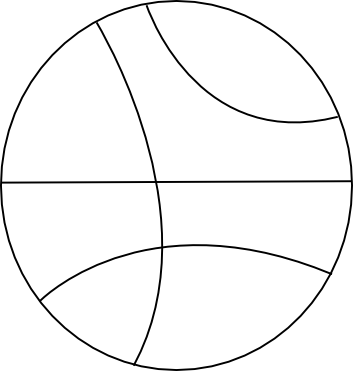
\includegraphics[width=0.5\textwidth]{PoincareDisc.png}
	\caption[A visualisation of the two dimensional Poincar\'{e} disc model containing four geodesics]{A visualisation of the two dimensional Poincar\'{e} disc model containing four geodesics \protect{\cite{poincare_model_web_page}}.}
	\label{fig:poincare_example}
\end{figure}

An example of this is shown in figure \ref{fig:poincare_example}. Here, four separate geodesics have been drawn on a hyperbolic plane and then visualised in Euclidean space using the disc model. Though these lines do not appear straight in Euclidean space the negative curvature of the hyperbolic space causes their apparent curvature in this model. Any geodesics which do not intersect inside the disc are considered parallel.

Measuring a Euclidean angle in this model yields the actual hyperbolic angle thus making the model conformal. Angles are determined by simply measuring the angle between the tangents of the Euclidean representation of the curves at the point of intersection. This property of the model makes it extremely useful for visualisations where angles are important.

Calculating hyperbolic distance in the disc model is more complex than simply measuring distances in the Euclidean representation. hyperbolic distance in the disc model, between the Euclidean points A and B, is defined as \cite{blair_inversion_2000}:

\begin{equation}
\label{distance_disc_model}
\log(AB,PQ)
\end{equation}

where P and Q are the ideal points of the geodesic that bisects A and B. These points must be in the order P, B, A, Q on the line. (AB, PQ) is the \textit{cross-ratio} of the four points and is defined as \cite{blair_inversion_2000}:

\begin{equation}
\label{cross_ratio}
(AB,PQ) = \frac{|AP|\cdot|BQ|}{|BP|\cdot|AQ|}
\end{equation}

where |PQ|, for example, is the Euclidean arc length between the points P and Q on the Euclidean representation of the hyperbolic line which intersects A and B.

The further an object is from the centre of the space the more compressed it's Euclidean representation becomes, making it appear smaller. Objects near the centre of the space are represented more accurately as the compression of the hyperbolic space is low there.

\subsection{The Beltrami-Klein Model}

The Beltrami-Klein model of hyperbolic geometry, known henceforth as the \textit{projective model} addresses the issue of the distortion of the "straightness" of lines but introduces a distortion of angle.

The projective model is again defined in two-dimensional Euclidean space as the open unit disc, given earlier in equation \ref{eq:open_unit_disc_eq}. A geodesic, in the projective model is any chord of the unit disc. Indeed, for a geodesic in the disc model which has ideal points A and B it is trivial to determine the equivalent in the projective model, it is simply the chord AB.

The method for calculating distance in the projective model differs slightly from the disc model and the distance between points A and B is defined as \cite{milnor_hyperbolic_1982}:

\begin{equation}
\label{distance_disc_model}
\frac{1}{2}\log(AB,PQ)
\end{equation}

Where P and Q are again the ideal endpoints of the geodesic that intersects A and B and all four points are defined on the line in the order P, B, A, Q. (AB, PQ) is the cross-ratio of the four points as defined in equation \ref{cross_ratio}.

\begin{figure}
	\centering
	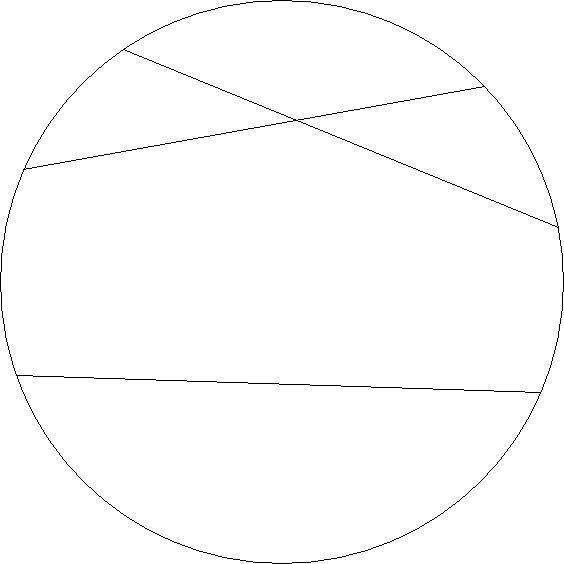
\includegraphics[width=0.5\textwidth]{Klein_model.png}
	\caption[A visualisation of the two dimensional Beltrami-Klein model containing three geodesics]{A visualisation of the two dimensional Beltrami-Klein model containing three geodesics \protect{\cite{klein_model_image}}.}
	\label{fig:klein_example}
\end{figure}

Figure \ref{fig:klein_example} provides an example of the model containing three geodesics. If two geodesics do not intersect within the  In this diagram the two topmost lines are parallel to the bottommost line and both pass through the same point, an important property of hyperbolic space. As the hyperbolic space is effectively bent in the visualisation, Euclidean angles in this model do not correspond to the same hyperbolic angles and this must be accounted for if the correct modelling of angles is important, as such the model is not conformal. Of course, if it is unimportant for angles to be accurate in the visualisation then this model may be ideal.

As the model is not conformal, it is difficult to measure hyperbolic angles given only the Euclidean representation of the model. Instead of attempting to measure angles directly, it is far more simple to convert to a conformal model and measure Euclidean angles directly. Fortunately, a simple conversion exists from the projective model to the disc model:

\begin{equation}
\label{projective_to_disc}
u=\frac{(1-\sqrt{1-s\cdot{}s})s}{s\cdot{}s}
\end{equation}

Where $s$ is a vector representing a point in the projective model and $u$ is its equivalent in the disc model. A similar conversion exists in the opposite direction and is given by:

\begin{equation}
\label{disc_to_projective}
s=\frac{2u}{1+u\cdot{}u}
\end{equation}

As the models are related by these simple equations conversion between them is trivial. Of course, any geodesic can be easily converted between the models by using its ideal points, simplifying conversion between the two models further.

It is important to note that both the disc and projective models map hyperbolic space to Euclidean space in such a way that changing the position of the centre of the visualisation will alter the Euclidean size of objects shown. This property effectively allows for a focus on a specific object, which will appear in the centre of the visualisation at its actual hyperbolic size but also gives a view of the entire space with objects being scaled down in size more the further they are from the centre. This property of these visualisations is extremely useful for displaying trees which have high branch factors, a property that is exhibited by graph representations of the internet.

\subsection{The Poincar\'{e} Half-Plane Model}

Both models discussed previously represent the infinite hyperbolic plane inside a finite Euclidean circle, the Poincar\'{e} half-plane model, known henceforth as the \textit{half-plane} model, does not. Instead, the infinite hyperbolic space is plotted in the upper-half plane, defined as \cite{kubo_geometry_1988}:

\begin{equation}
\label{upper_half_plane}
\{(x,y):y>0\}
\end{equation}

Unlike the previous two models, the half-plane model is unbounded in the x direction, providing infinite space in which to visualise hyperbolic space. However, a bounding still exists in the y direction, which, like previous models, compresses the space infinitely at the bound. Ideal points lie on the line $y=0$ which are again infinitely far from all other points.

As the space is infinite in the x and positive-y directions geodesics appear quite differently to the disc and projective models. A geodesic in the half-plane model appears as either a Euclidean circular arc perpendicular to the x-axis or as a straight line perpendicular to the x-axis. Lines are parallel if they do not intersect in the plane.
\begin{figure}
	\centering
	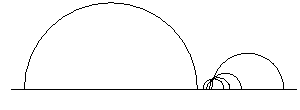
\includegraphics[width=0.75\textwidth]{upper-half-plane.png}
	\caption[A visualisation of the two dimensional Poincar\'{e} half-plane model containing five geodesics]{A visualisation of the two dimensional Poincar\'{e} half-plane model containing five geodesics \protect{\cite{half_plane_example}}.}
	\label{fig:half-plane-example}
\end{figure}

Figure \ref{fig:half-plane-example} shows an example of the half-plane model in which five geodesics have been plotted. In this example all of the lines on the right are parallel to the leftmost line, additionally the lines on the right also intersect at a single point.

Measuring the distance between points in the half-plane model is more complex than the previous two and is defined as \cite{kubo_geometry_1988}:

\begin{equation}
\label{half_plane_distance}
arcosh\left(1+\frac{(x_2-x_1)^2+(y_2-y_1)^2}{2y_1y_2}\right)
\end{equation}

Where the points are given in the form $(x_1, x_2), (y_1, y_2)$, unlike the previous models which use pure vector mathematics. Measuring angles is simple, however, as the model is conformal, simply measuring the Euclidean angle between the tangents of the lines at the point of intersection yields the hyperbolic angle.

An interesting property of the half-plane model is the appearance of circles in the model, they appear as Euclidean circles. Though this may seem strange the appearance of the circle is deceiving as its hyperbolic centre is not equivalent to its Euclidean centre. A hyperbolic circle with centre $(x,y)$ and radius $R$ is modelled by a Euclidean circle with centre $(x, y \cosh R)$ and radius $y \sinh R$. This conformance of circles makes the half-plane model a good choice for representations which include hyperbolic circles, but one must be wary of the distortion of the centre of such circles.

\section{Embedding Methods}
In order to be able to produce a visualisation of hyperbolic space it is first necessary to determine how the chosen data lies in such a space. This process is known as \textit{embedding} and will be discussed in this section.

\subsection{A Greedy Embedding Method}

Cvetkovski et al. \cite{cvetkovski_hyperbolic_2009} describe a method for embedding dynamic graphs into hyperbolic space for the purposes of routing. This implementation uses the Poincar\'{e} disc model. Focussing on trees, this method selects a root location in the space at which to place the root node of the tree subject to constraints which cause the node to be placed at an optimal location in the space. The method relies on the network nodes themselves electing a root node and subsequently forming a minimal-depth tree. The nodes accomplish this by each selecting a parent node to be the node that is the closest in hops to the root node. 

After the nodes have identified their parents, the root node is plotted into the space at the chosen location and each node calculates its position in the embedding relative to its parent node. This calculation is performed by initialising two angles for the root node $\alpha_r = \pi$ and $\beta_r = 2\pi$ which correspond to ideal points. A node, $n$, to be placed in the embedding receives angles $\alpha_n = \alpha_p$ and $\beta_n = (\alpha_p + \beta_p) /2$ from its parent, $p$, and determines its own position in the embedding by reflecting the position of it's parent (in this case the root node) in the geodesic $G$ constructed between $\alpha_n$ and $\beta_n$ After sending $\alpha_n$ and $\beta_rn$ to the child the parent node updates the value $\alpha_p := \beta_n$. This method of updating these values ensures there is unlimited space available for the expansion of the tree. This process in then repeated for each node to form a greedy embedding. 

This method of creating an embedding, while offering guaranteed success due to its greedy implementation, has some flaws. The real, physical locations of the nodes are not represented in the embedding, something which is important to the aims of this project. Further, the embedding is designed to be used for a greedy routing algorithm described in the same work, which limits its usefulness when applied to the problem for this project. Indeed, the embedding produces a tree which is not indicative of all links between all nodes and would therefore misrepresent the data. Despite these flaws, the approach of performing an embedding in this way is an interesting application of knowledge and does give some useful insight into the practical uses for such embeddings. 

\subsection{H3: Large Directed Graphs in Hyperbolic Space}

Munzner \cite{munzner_h3_1997} describes a method for laying out large directed graphs in hyperbolic space. This implementation uses a three dimensional version of the Beltrami-Klein model. The method once again operates on trees but it is possible to display further links between nodes once the model has been plotted. Though a root node must be chosen and a spanning tree constructed, it is possible to use this method to visualise an undirected graph accurately. 

The basis of the method uses \textit{spherical caps} to lay out the nodes in the hyperbolic space. Each node has a cap with size proportional to the number of nodes descended from it in the tree. This includes all descendant nodes, not just immediate child nodes. These caps represent the area required to embed all descendant nodes of the node to which the cap belongs. As hyperbolic space expands in all directions, it is possible to fit more caps of equivalent size into the space further down the tree. This allows trees with high branch factor to be embedded into the space easily.

The algorithm to place the caps functions recursively; it first computes the size of the caps required for all leaf nodes, which have a fixed cap size due to having no children, which is the base case for the algorithm. The algorithm then traverses back up the tree and computes the area required for the cap belonging to each node, taking into account the cap size of all child nodes. Finally, the cap size for the root node is calculated, which is the total size of the embedding. Though the size of the caps has been calculated at this point, they have not been laid out in the space, this is the next function of the algorithm, which iterates down the tree from the root node laying out each child cap of each node, until all caps have been placed. This is accomplished through \textit{sphere-packing}, a common mathematical problem outlined by Hales in 1992 \cite{hales_sphere_1992}.

While this method seems more appropriate than the previous one, it does present issues when combined with the aims of this project. Once again, the embedding does not take into account the physical locations of the nodes, indeed the examples supplied in the paper are those without such locations like files in a file system. Though the method could be adapted to take physical location into account, it would be far more appropriate to use a method designed to do this from the beginning. Though it may appear that it is possible to embed a graph using this model the embedding would distort the distances between the nodes even if it was converted to account for physical location. Due to the original embedding being constructed using the tree any links which did not appear in this tree would be vastly distorted, making the embedding misleading. Though the technique of using spherical caps and sphere packing to perform the embedding is efficient, the limitations of this method as a whole decrease its viability for use in this project.

\subsection{A More Mathematical Embedding Method}
\label{sec:hyperbolic_embedding}

So far, the methods discussed to perform an embedding have been of the practical, algorithmic variety. The method outlined by Wilson et al. \cite{wilson_spherical_2014} is a more mathematical method. This method uses the matrix describing the distances between points in Euclidean space, which should correspond to the distances in hyperbolic space, to produce a embedding of points in hyperbolic space.

This method uses the inner product of the points, defined for hyperbolic space as: 

\begin{equation}
\label{eq:inner_product_hyperbolic}
\langle x_i,x_j\rangle = -r^2\cosh \left(\frac{d_{ij}}{r}\right)
\end{equation}

where $r$ is the radius of the embedding space and $d_{ij}$ is the distance between a pair of points $i$ and $j$. It is possible to calculate $\boldsymbol{Z}$, the inner product of the points, directly from this equation, but this is not possible immediately as the radius, $r$, is unknown. As $\boldsymbol{Z}$ is an inner product matrix of points in hyperbolic space it should have exactly one negative eigenvalue and one zero eigenvalue. This is due to hyperbolic space having a single negative dimension. Knowing this, it is possible to minimise the magnitude of the second smallest eigenvalue to find $r$ by:

\begin{equation}
\label{eq:argmin_hyperbolic}
r^*=\underset{r}{\arg\min}|\lambda_2[\boldsymbol{Z}(r)]|
\end{equation}

where $\lambda_2$ is the value of the second smallest eigenvalue of $\boldsymbol{Z}$. Having approximated $r$ it is then possible to calculate $\boldsymbol{Z}$ using equation \ref{eq:inner_product_hyperbolic}, this then allows for the calculation of $\boldsymbol{X}$, the point matrix for a Euclidean embedding of the space, through eigendecomposition of $\boldsymbol{Z}$ to obtain a matrix of its eigenvalues, $\boldsymbol{\Lambda}$ and a matrix of its eigenvectors $\boldsymbol{U}$. It is then possible to calculate $\boldsymbol{X}$ by:

\begin{equation}
\label{eq:embedding_x}
\boldsymbol{X}=\boldsymbol{U}_Z\boldsymbol{\Lambda}_{z||}^{\frac{1}{2}}
\end{equation}

The result of this equation is an $NxN$ matrix for which each row is a point and each column represents a dimension of the embedding. As with a standard embedding, it is possible to drop any dimensions which have negative eigenvalues, yielding a co-ordinate matrix that specifies the hyperbolic co-ordinates of the points.

This method is vastly superior to those previously discussed, its primary advantage arises from the strategy of embedding using pre-existing geometric data. In the case of this project, this allows the embedding to use location data gathered for ASes without having to adapt the embedding method. Further, this method is already generalised to any number of dimensions, meaning it is possible to produce both two and three dimensional representations of the data. 

\section{Haversine Formula}
\label{sec:haversine}
When considering the locations of ASes on the Earth's surface a suitable system must be used, the most obvious and simple of which is the latitude longitude geographic co-ordinate system (henceforth known as lat-long). As this system can effectively map any point on the Earth's surface and is well known and understood it is an easy choice to make. However, a key requirement of the chosen system is that it is possible to easily determine distances, something which lat-long fails to provide. It is insufficient to simply treat the lat-long co-ordinates as absolute positions and calculate distance through the difference between the co-ordinates as the earth is not flat. Instead a method known as the Haversine formula must be used.

The Haversine formula calculates the distance between two points on the surface of a sphere and is defined as \cite{chopde_landmark_2013}:

\begin{equation}
\label{haversine_formula}
2r\sin^-1\left(\sqrt{\sin^2\left(\frac{\phi_2 - \phi_1}{2}\right) + \cos(\phi_1) \cos(\phi_2) \sin^2\left(\frac{\psi_2 - \psi_1}{2}\right)}\right)
\end{equation}

where a pair of points are given with latitude and longitude $(\phi,\psi)$ and $r$ is the radius of the Earth. 

Though the computed distance may not be exact due to the Earth not being a uniform sphere, it is satisfactory for the purposes of this project.
\part{Design and Methodology}
\thispagestyle{empty}\cleardoublepage
\label{sec:design}
\chapter{Methodology}

As this project aims to produce some software a discussion of the methods that will be used to produce this software is necessary. This section aims to outline the methods that will be used when writing software for this project.

\section{Development Method}
Writing software is a complex process which cannot be accomplished by just writing code. Instead, there are frameworks which provide a set of rules which aim to streamline development. 

\subsection{Waterfall Model}
One such methodology is known as the \textit{waterfall model} \cite{royce_managing_1970} and describes an iterative method for developing software. The main approach for this model is to perform the following in order:

\begin{enumerate}
	\item{Requirements}
	\item{Design}
	\item{Implementation}
	\item{Verification}
	\item{Maintenance}
\end{enumerate}

In terms of this project, several of these do not apply. Requirements are not required as the software is not a deliverable, indeed, there is no customer to propose requirements or to verify they have been met. The \textit{requirements} of this project are effectively implicit in the aims, described in section \ref{sec:aims}. Again, as no product is being delivered to a customer the maintenance step is not required. 

The iterative process described by this model does not necessarily work well when applied to this project. As the steps must be completed in order the system design must be completed before any work on the implementation can begin. If any issues arise in the implementation stage then the design stage must be revisited, slowing development. Indeed, the same applies to the verification stage, if any issues arise in testing then either the implementation or both the design and implementation must be modified. The waterfall model is much more suited to large software projects which must be delivered to customers.

\subsection{Agile Development}

Agile development \cite{agile_manifesto} is a set of software development methods which aim to provide adaptive planning and a rapid response to change. Agile development does not provide a rigid framework to follow when undertaking development, instead it operates through the use of principles which guide development appropriately. 

A key principle of agile development is that the processes used must be robust to changing requirements, if issues are detected at any stage of development then they must be handled within that stage. It is pointless modifying the design when a small bug is encountered during implementation, and agile protects from this. Using agile development for this project allows for easy adaptation if such problems occur. 

As the program produced for this project is not part of the deliverables there is no need to produce documentation for it. Agile development supports this decision, as it mandates that concrete design decisions should not be made before it is understood how they can be implemented. For this reason, the design and implementation of this project will be performed in parallel. This allows any changes in design to influence implementation quickly. Software produced can also be tested as it is implemented, another philosophy of agile development.

Overall, agile development would appear to be a good choice for use in this project, due to its synergy with the project aims and its simplistic development model.
\chapter{Design and Implementation}
\label{cha:Design}

\section{Platform and Programming Language}
\label{sec:DesignLanguage}
As this project aims to produce visualisations of the internet embedded in hyperbolic space it must employ some existing technologies to do so. This section will discuss which technologies will be used and will justify their use. 

The most important technical decision to be made is the choice of programming language as it affects how the project will be designed and limits possible techniques. The following languages will be considered for use in this project:

\begin{itemize}
	\item{MATLAB}
	\item{Python}
	\item{Java}
\end{itemize}

\subsection{MATLAB}
MATLAB \cite{MATLAB:2015} is a high level mathematical programming language which is provided with an environment. It excels at mathematical programming as it provides many high level functions designed to perform calculations. MATLAB provides matrix and vector support as standard. As this project will require some complex mathematical operations it would seem that MATLAB is the ideal choice, however it does have limitations which affect its viability. 

MATLAB is a commercial product, and is not free, requiring payment in order to use the software. The University of York does provide MATLAB on university owned PC's, however it is currently not possible to install this provided version on a personal PC, where most of the work for this project will be undertaken. Additionally, MATLAB has relatively few third party libraries and if functionality for a specific task does not exist in the language it would most likely be necessary to develop it from scratch.  It is unlikely that MATLAB will have the necessary third party libraries for collecting the data to be used in this project. Due to these limitations it would seem that MATLAB is not a suitable candidate for this project.

\subsection{Python}
Python (\textit{www.python.org}) is a multi-platform programming language which boasts one of the largest sets of third party libraries of any language. This, combined with the speed of its native C implementation makes it an ideal choice for this project. Python comes pre-installed on many operating systems and is available on all popular platforms.

Unlike MATLAB, python does not provide any mathematical matrix or vector support as standard, but does provide array functionality through "lists". Fortunately, as python is so widely used it has many third party libraries which provide mathematical functions, such as NumPy \cite{python_numpy_2015} and SciPy \cite{jones_scipy:_2001}. These libraries provide functionality similar to MATLAB while still allowing the flexibility of a general programming language.

\subsection{Java}
Java (\textit{www.java.com}) is a multi-platform programming language which compiles programs to run on a virtual machine known as the JVM. Java has wide support with many third party libraries and runs on many platforms. As all code is executed on the JVM, programs need only be compiled once and will run on all platforms for which a version of the JVM exists. 

Though Java is natively multi platform, this feature is not actually useful in the scope of this project as it will only be run on a single platform. Additionally, as compiled Java code is interpreted by the JVM and is not native machine code, the general performance of the language falls below native languages.

Due to the limitations of Java and MATLAB this project will be written in python, making use of NumPy, SciPy and any other third party libraries which may be necessary.

\section{Data Sources}
\label{sec:DesignDataSources}
As the primary aim of this project is to create and visualise an embedding of the internet it is necessary to collect data describing its structure, on which to base the embedding. Using Autonomous Systems as the subject of the mapping serves to make data collection easier, however the following data is required for each system if an embedding is to be created:

\begin{itemize}
	\item{Organisation and ID}
	\item{Relationships between Autonomous Systems}
	\item{Location}
\end{itemize}

\subsection{Organisation and ID}
Though it may seem trivial, finding a dataset which contains a mapping of Autonomous System Numbers (ASNs) to the organisation that owns them was not straightforward. At first attempt, the use of the program \textit{whois} was considered as it is possible to query it with an ASN in order to retrieve the owner as well as further data which could have been used to identify relationships between ASes. However, upon testing several queries it became clear that the information provided by \textit{whois} was not consistent across RIRs. Further, executing an external program, which requires an internet connection, for each AS would add a large amount of overhead to the application. 

If it was not possible to connect to the internet to retrieve the data for each AS individually then a pre-compiled dataset is required. Of course, if a database could be found that contains all required data then the choice would be simple, however no such database exists. Instead, each piece of data described earlier must be obtained from separate databases. 

In order to begin enumerating ASes a dataset which contains the ASNs for all systems must be used. There are several web pages (for example \textit{bgp.potaroo.net/cidr/autnums.html}) which simply list all known ASNs along with their organisation, however the system through which this data is collected is unclear and the formatting of the web pages makes them difficult to parse. 

Clearly, some form of downloadable database is required which would allow the application to have fast access to all available AS data. One such dataset is provided by the Center for Applied Internet Data Analysis (CAIDA) and contains several different files which provide both ASN and organisation data \cite{org_mapping_caida_2015}. Further, this data is provided for free to educational users. The files themselves are simply text files which can be parsed easily in Python. The method through which the data is collected is clearly outlined on the website as well as how often new data is published. This dataset provides a reliable way of enumerating ASes and finding to which organisation they belong.

\subsection{Relationships between Autonomous Systems}
Without data describing the relationships between ASes it would not be possible to create an embedding. Collecting this data will allow the physical connections between ASes to be determined, which, when used in conjunction with location data, provides enough information to calculate the distances between connected ASes.

Again, use of the \textit{whois} application was considered but the flaws of this method definitely outweigh its advantages. Again, CAIDA provides a convenient dataset named \textit{AS Relationships} \cite{relationships_caida_2015} which contains the inferred relationships between ASes where each relationship represents a physical connection. This dataset is provided free for educational use and contains a text file which can be easily parsed in Python. 

\subsection{Location}
Determining the geographical location of an AS provides a way to determine distances between ASes, an operation which is required in order to create an embedding. Upon searching for a dataset which contained the locations of all ASes it became apparent that no such dataset existed. This was primarily because an AS does not have a single location, it is possible for an AS to span a very large geographic area. This issue caused a significant setback in the projects design, how would it be possible to retrieve location data for an entity which does not have a singular location?

When considering the solution to this problem it became apparent that in order to retrieve location data for an AS it needed to have a component for which a location could be determined. Physical internet components such as routers have a defined location, and each component can be identified by its IP address.

Having determined that it is possible to determine a location for an IP address the next step is to find an IP address for an AS. This is not as simple as using a service to perform a lookup as there are no providers for this type of data. There is, however, a Python module which provides IP to ASN lookups known as pyasn \cite{asghari_pyasn_2014}. Though this may not seem useful it is possible to use the module to perform a reverse lookup for all known IP addresses in a specific AS. This module operates by providing functions to parse the current BGP table, converting it into a format which can be read by pyasn. This data is then used to perform lookups for which IP addresses route to which ASN.

Once this list of IP addresses is obtained it is then possible to determine the location of one of them. This can be done through the use of an IP geolocation service. Python bindings exist for many of these services, of which MaxMinds GeoIP \cite{python_geoip_2014} is one. This library contains functionality for downloading a database ahead of time for fast access. As all of the data required for this project is available locally on disk, the initial start up of the application should be significantly faster. 

\section{Further Data Considerations}

This section aims to outline any further data considerations which were raised during development of this project.

\subsection{Dataset Size}

Upon inspecting the datasets chosen for this project it became apparent that volume of data available was very large. Due to the calculations that must be performed in order to create an embedding a very large amount of memory is required. This is not feasible as access to a machine with enough RAM is not possible, therefore one of two workarounds must be employed: either store the data somewhere other than RAM or reduce the size of the data. 

The specific point in the application at which the data becomes very large will occur when calculating the distance matrix for all ASes. This matrix will be square with dimensions equal to the number of ASes. Attempts must be made to reduce the size of this matrix or the aims of the project cannot be fulfilled.

Storing the data outside of RAM would seem difficult in this case, but it is possible. In order to implement such a system in Python, a technology called Hierarchical Data Format (HDF) can be used. This allows for the creation of disk backed variable storage within Python that acts as though the object is stored in RAM. Access to the data would of course be slower than traditional variables but RAM is no longer a constraint. However, as the data being stored is a matrix it must support all of the numpy matrix operators. While the Python bindings for HDF (h5py) do support numpy, they do not support performing matrix operations on data backed by HDF. HDF is not a viable candidate to solve this problem for this reason.

While moving the data out of RAM may seem like a convenient solution, it is impossible to maintain compatibility with numpy while performing such an abstraction. Instead it would be easier to attempt to minimise or compress the data.The scipy library contains a \textit{sparse} matrix class which is effectively compressed and performs very well on matrices which contain many occurrences of the same value. Unfortunately, it is extremely inefficient to modify such a matrix heavily once it has been created which is a feature required for the construction of an embedding. 

Having exhausted all other lines of enquiry it is necessary to consider using a smaller dataset than initially intended. Unfortunately, this is not as simple as only using the first 1000 ASes, for example, as it is possible (though unlikely) for no relationships to exist between any of those ASes. Instead, the subset must be chosen carefully so as to eliminate any ASes which have zero links to the rest of the subset. One system which could be used to achieve this would be to follow the links from a specific AS to a set depth and use all ASes found as a subset. This could be implemented recursively and would provide a consistent way to generate small subsets of the main dataset.

\subsection{Data Availability}
While the chosen data sources contain relatively complete data for most ASes it is impossible to have full coverage. Of particular note is the unavailability of an IP address for some ASes. This is due to these systems having no IP address ranges which route to them, which is fairly common. Unfortunately, if it is not possible to determine a valid IP address for an AS it is not possible to determine its location. If an AS has no known location it cannot be part of the embedding as its distance from other ASes cannot be calculated. 

For this reason, it is necessary to validate the dataset before it is processed by removing any AS for which there is incomplete data. While this may seem an extreme measure there is no alternative as any ASes which have missing data are useless in this context. Further, performing this validation before the data subset is generated means that any ASes which are eliminated cannot be followed by the recursive algorithm. This effectively prevents any ASes which may have been orphaned from being included in the embedding, which prevents misleading information from being shown in the visualisations. 

\subsection{Organisation of Data}
As each AS has a large amount of associated data, it will be necessary to produce a method of organising this data so that it can be used effectively. It may be possible to simply encode the data for each AS into a list, and implement a rule for extracting data from these lists. For example, the ASN is at index $0$ and the name at index $1$. Unfortunately, this solution does not scale well when each object contains numerous data. Further, ASes are identified by their ASN and python lists by an index beginning at zero, these two indexing systems are not compatible as gaps exist in the allocation of ASNs. 

It seems that there are two separate problems here which must be solved in conjunction. Firstly, the issue of storing the data for each AS; a sensible way to solve this would be to define a custom python class which holds all of the data for a single AS. It is then possible to easily extract a specific piece of AS data from an AS for which the class object is known. 

The second problem, regarding the indexing of ASes is also simple to solve. Python has a built in dictionary structure \textit{dict} which allows for the referencing of its contents through a hashable key. Storing each AS class object in a dict with the ASN as the key would allow any AS to be located and any piece of data for that AS to be extracted. It is important to note that the ASN is being stored as a string in this instance, as it has no numerical meaning and arithmetic should not be performed on it. 

Though most of the data associated with an AS is singular, the location or name for example, there is a special case in the connections between ASes. As the network of ASes can be represented as a graph this structure must be described by the stored data. A simple way to achieve this is to store a list of the ASN for all ASes connected to an AS. This method provides a way to retrieve all connections to an AS easily, by simply extracting the list and a way of following these connections through the main AS dict, using the ASNs. If, however any more information was to be stored about a particular AS to AS relationship, such as whether that link is peer-peer or provider-customer, then a new \textit{peering} class can be created which facilitates the storage of such data. 


\section{Performing The Embedding}

The method discussed previously in section \ref{sec:hyperbolic_embedding} will be used to perform the embedding for this project. This method requires a distance matrix to operate upon which can be obtained from the AS location data using the Haversine formula (discussed in section \ref{sec:haversine}). The method itself could be implemented in python, however an implementation already exists in MATLAB, which is the better choice as this implementation has been proven to work, and allows more development time for other parts of the project. 

\subsection{MATLAB in Python}

As this implementation is not native python and cannot be run as such, there are two choices for how to proceed. The simplest choice, though it is inelegant, is to export the distance matrix from python, import it into MATLAB, run the embedding procedure manually and transfer the results back. While it is simple, this method is extremely time consuming, as the manual transfer and execution significantly slows down runs of the overall application. Additionally, as this method is not automated it is possible that mistakes will be made when copying the data back and forth. 

Instead of manually transferring the data back and forth, it could be transferred automatically, by python, when the embedding procedure is required to be run. This solution eliminates the introduction of random error at the point of copying and decreases the running time of the application. Unfortunately, this method still requires the MATLAB embedding code to be invoked manually. There is, however, a third way. If it were possible to execute a MATLAB instance from inside python, and transfer data in and out of this instance then the entire solution could be completely automated.
Fortunately, a python library exists to solve this problem. A project named \textit{matlab\_wrapper} (\textit{github.com/mrkrd/matlab\_wrapper}) allows for the invoking of a MATLAB session from within python with functions to import and export data and execute arbitrary MATLAB code. With this library the entire embedding process can be automated, significantly speeding up the time required to produce visualisations. 

\subsection{Calculation of Embedding Points}

Though it is now possible to execute the code for the embedding, this does not produce the final embedding co-ordinates, only the inner product matrix, $\boldsymbol{Z}$, of the points. The steps to perform this conversion are discussed mathematically in section \ref{sec:hyperbolic_embedding} and will be discussed in terms of implementation here. 

The equation that must be implemented is:
\begin{equation}
\label{eq:embedding_x_impl}
\boldsymbol{X}=r\boldsymbol{U}_Z\boldsymbol{\Lambda}_{z||}^{\frac{1}{2}}
\end{equation}

where $r$ is the radius of the space, and $\boldsymbol{U}$ and $\boldsymbol{\Lambda}$ are the eigenvectors and eigenvalues of $\boldsymbol{Z}$ respectively. In order to implement this, the eigenvalues and eigenvectors of $\boldsymbol{Z}$ must be calculated. The linear algebra package of SciPy provides functionality to do this, and, as $\boldsymbol{Z}$ is symmetric (due to the inner product being commutative) it is possible to use the efficient \textit{eigh()} function designed for Hermitian or symmetric matrices. As an interesting side node, the standard \textit{eig()} function will not detect if a matrix is Hermitian or symmetric and will return complex values in any case. 

Having calculated the eigenvectors and eigenvalues of $\boldsymbol{Z}$ it is possible to calculate the value of $\boldsymbol{X}$ directly using equation \ref{eq:embedding_x_impl}. As the matrix values in this equation will be stored in NumPy arrays the implementation is simple, and the standard python multiplication function suffices. However, the standard python $\textit{sqrt()}$ does not support NumPy arrays and the NumPy equivalent must be used. As the magnitude of the eigenvalue matrix is required the NumPy \textit{absolute()} function must be used to prevent complex numbers being returned by \textit{sqrt()}.

Though $\boldsymbol{X}$ is able to be calculated, this does not yield the co-ordinates straight away. A further step is required in order to extract the correct dimensions. The eigenvalues of $\boldsymbol{Z}$ each correspond to a column in $\boldsymbol{X}$, this allows for the determination of the correct dimension columns as there will be a single large negative eigenvalue (the negative dimension of the space) and $N$ large positive eigenvalues (the positive dimensions of the space). All other eigenvalues should be have small magnitude compared to these. Finding the correct indexes for the dimensions is simple, the eigenvalue array must be sorted in ascending order. The eigenvalue, $\lambda^-$ for the negative dimension will then be at index 0 in the sorted array. The correct column in $\boldsymbol{X}$ can then be determined by finding the index of $\lambda^-$ in the eigenvalue matrix of $\boldsymbol{Z}$. The $N$ positive dimensions can be located in a similar fashion, though these will be located at index $-N$ for $N=1,...,n$, in the sorted eigenvalue array. It is then trivial to extract the correct columns from $\boldsymbol{X}$ and create co-ordinate tuples for each point in the embedding. For a three dimensional hyperbolic space four embedded dimensions are required as it is embedded in a higher dimensional space, the implications of this will be discussed in the next section.

\subsection{Conversion to the Ball Model}

Though it has not been discussed, there is a further model of hyperbolic space known as the hyperboloid model. This model represents $N$-dimensional hyperbolic space in an $N+1$-dimensional space. Of course, the hyperbolic data in this project is in three dimensions, producing a four dimensional embedding, which is impossible to imagine in three dimensional space. Instead the embedding must be projected into three dimensional space in order to be able to produce meaningful visualisations. 

The Poincar\'{e} disc model, discussed earlier in section \ref{sec:discmodel} is a two dimensional representation of hyperbolic space, represented in two dimensional Euclidean space. There is a three dimensional version of this model, in which the disc is expanded into a sphere, and which represents three dimensional hyperbolic space. The model has similar behaviour as its two dimensional counterpart and is known as the \textit{Ball model}. Having the point data in this form would greatly simplify conversion to the other two models discussed in section \ref{sec:LitReviewVisHyperbolic}. 

In order to convert the four dimensional hyperboloid model to the three dimensional Ball model, it is necessary to project the higher dimensional space onto the lower one. In this case if the projection is through the point $(-1, 0, 0, 0)$ it will produce coordinates in the Ball model. This projection can be performed for a four dimensional point $\boldsymbol{x}$ as follows:

\begin{equation}
\frac{1}{x_0 + 1}
\begin{pmatrix}
x_1 \\
x_2 \\
x_3 \\
\end{pmatrix}
\end{equation}

Implementing this in python is trivial using NumPy and looping through each co-ordinate. After the projection has been performed it is possible to plot the returned co-ordinates in three dimensional space. 

\section{Displaying Visualisations}
As the aim of this project is to produce visualisations it is necessary to perform some kind of 3D graphics programming. As co-ordinates in three dimensions have already been obtained the conversion to a visualisation should be trivial. A choice must be made, however, regarding the library to use for the graphics programming. 

There are multiple methods through which to produce a 3D visualisation in python, some of which are more flexible than others. If the points themselves are treated as generic data it is possible to use the python plotting library \textit{matplotlib} to produce a static plot of the data. This method is simple, but lacks flexibility, the plot cannot be rotated and the axes are fixed. Instead of using a method designed for visualising data, it would be better to treat the data as visual information and use a full 3D graphics library. 

There are many choices available for such 3D programming within python, one of which is VPython (\textit{vpython.org}). VPython is a python distribution that comes with the python module \textit{visual} pre installed. This module allows for flexible 3D graphics programming through an IDE named VIDLE. Though it may seem ideal, this solution is aimed at those wishing to experiment with this type of programming, being restricted to the IDE supplied with the distribution is not ideal as the application being produced does not only contain graphics programming. Further, there is no native Linux version of VPython and this project is being developed on Linux. 

Instead of concentrating on how to use python to produce visualisations it would be more sensible to seek to produce the best visualisation possible and then consider how to do this using python. VTK \textit{www.vtk.org} is an open-source software system for 3D computer graphics. VTK is written in C++ but has bindings in python and other languages. As it is compiled to native code it is fast and compatible with any operating system. This is a good choice for this project as it provides the flexibility required and enables the visualisation to be created directly from python.

The actual process of displaying visualisations will not be discussed here as it is effectively boilerplate and not interesting considering the domain of the project. 

\part{Results}
\thispagestyle{empty}\cleardoublepage
\label{sec:results}
\chapter{Initial Findings}
As the aim of this project is to produce visualisations and navigate these this section will demonstrate some of the visualisations produced and make comparisons between them. All of the visualisations will be produced with a reduced dataset generated using the method described in section \ref{sec:dataset_size}. The method will be run with a root of AS1 and a search degree of 3. This produces a graph of 1327 ASes. The visualisations themselves represent each AS as a square point with the origin represented as a larger point.  It is important to note that these visualisations are 3D and are difficult to fully appreciate on paper. Two dimensional visualisations will not be generated as the data is drawn from three dimensional Euclidean space, and would not be represented well by them.

\section{Disc Model Visualisation}

\begin{figure}
	\label{fig:disc_no_hyperbolic}
	\centering
	\includegraphics[width=0.75\textwidth]{disc_no_hyperbolic}
	\caption{A visualisation of a subset of the internet in the ball model.}
\end{figure}

Figure \ref{fig:disc_no_hyperbolic} shows a visualisation of the generated subset of ASes in the ball model. This visualisation shows the geographical structure of the internet very well with the centre of the diagram showing the outline of the USA very clearly. The model is not perfectly spherical most likely due to mismatches in the location data between IP addresses and actual AS locations. The method has successfully embedded the data given into hyperbolic space, but the properties of the space itself have not been exploited. As the initial data is drawn from Euclidean space it is represented accurately without the need for hyperbolic space. It would seem that some tweaking of the input data is required for this model.

\section{Projective Model Visualisation}

\begin{figure}
	\label{fig:klein_no_hyperbolic}
	\centering
	\includegraphics[width=0.75\textwidth]{klein_no_hyperbolic}
	\caption{A visualisation of a subset of the internet in the projective model.}
\end{figure}

Figure \ref{fig:klein_no_hyperbolic} shows a visualisation of the generated subset of ASes in the projective model. Once again the physical structure of the internet is well represented but the shape is distorted for the same reasons. This visualisation is remarkably similar to the ball model from figure \ref{fig:disc_no_hyperbolic} due to how the two models represent hyperbolic space in the unit ball. Indeed, as the only difference between these models is how the space is bent there should be little difference between them. Again, this model does not show anything that cannot be shown using Euclidean space.

An interesting note about both the ball and projective models 

\section{Half-Plane Model Visualisation}

\begin{figure}
	\label{fig:upper_no_hyperbolic}
	\centering
	\includegraphics[width=0.75\textwidth]{upper_no_hyperbolic}
	\caption{A visualisation of a subset of the internet in the half-plane model.}
\end{figure}

Figure \ref{fig:upper_no_hyperbolic} shows a visualisation of the generated subset of ASes in the half-plane model. This model produces very different results to the others but still shows the physical structure of the internet, though it is more difficult to make out. The USA is visible as a dense patch of ASes in the middle of the main set. An interesting note is how far from the origin the ASes are translated in this model, whereas in the previous two it was inside the \textit{sphere} they formed. This translation makes the model somewhat less useful for showing this type of data. Indeed, the other two models are much better as they are represented in the unit ball to begin with.


\chapter{Adjustments to the Embeddings}

\section{Adjusting the Data}
\label{sec:adjusting}

It would seem that while the embedding and visualisation techniques work, the data itself is not appropriate for display in this way. This is due to it being drawn from Euclidean space originally; the data cannot possibly require a hyperbolic space to be visualised properly. As this results section aims to demonstrate that useful visualisations can be produced it is necessary to perform some modification to the input data which causes useful visualisations to be produced. 

One such modification could be made to the distance matrix itself, though the distances are being drawn from euclidean space it is possible to use information about each AS to augment this data to produce a distance matrix which can only be represented in hyperbolic space, or would be better represented in this way. It has been established that the hierarchical nature of the internet is what makes hyperbolic space a good candidate for representing it, therefore adding some measure of the difference in hierarchical level of the ASes to the distance matrix could produce some useful results. 

Given the available data it is possible to calculate the difference in degree between ASes, which gives an indication in their tier separation as higher tier ASes tend to link to many lower tier ASes which in turn link to fewer ASes themselves. By subtracting a factor of degree separation from the distance calculation higher-tier ASes are effectively pulled nearer to the origin of the space. This effect occurs due to there being less space to cover near the origin in hyperbolic space coupled with the distance measurement being smaller for ASes of vastly differing degrees. 

\begin{figure}
	\label{fig:distance_new_klein}
	\centering
	\includegraphics[width=0.75\textwidth]{distance_new_klein}
	\caption{A visualisation of a subset of the internet in the projective model with a modified distance calculation that accounts for degree separation.}
\end{figure}

Figure \ref{fig:distance_new_klein} shows a visualisation of the generated subset of ASes in the projective model, which uses this new distance calculation. The USA is visible on the left of the image and clearly some higher degree ASes have been \textit{pulled} further towards the origin. As these nodes represent the important backbone of the internet this visualisation is very useful; it gives a geographical view of where the high degree nodes on the internet reside while also representing how important they are in their distance from the origin. 

This modification is extremely important for the aims of this project as it has produced a useful visualisation of the internet which uses the properties of hyperbolic space to show more information than can be shown easily in Euclidean space. 

\section{Adding AS Links}
\label{sec:adding_links}

Though data was collected about the links between ASes it has not been used in any visualisation yet. As this data is available it would be unwise to simply ignore it. The AS links will be added to the visualisation generated in section \ref{sec:adjusting} as this is the most interesting visualisation generated. 

\begin{figure}
	\label{fig:with_links}
	\centering
	\includegraphics[width=0.75\textwidth]{klein_with_links}
	\caption{A visualisation of a subset of the internet in the projective model with links between ASes shown.}
\end{figure}

Figure \ref{fig:with_links} shows a visualisation of the generated subset of ASes in the projective model, with links between ASes shown. Peer-peer connections are shown in red and provider-customer connections are green. While the addition of the links does add more information to the visualisation; it makes it very difficult to see the most important ASes which reside near the origin. Though some ASes with very high degree are visible due to the sheer number of links they have.

Instead of augmenting the visualisation the links actually do more to expose its flaws. In the top right of the image there is a peer-peer link that terminates at an AS which appears to have no other links. This is an odd depiction as surely this AS must have some customers if it has a peer-peer link with another AS? This has exposed a flaw in the method used to generate the subset of ASes for embedding. As this method follows the links from a chosen root node for a number of \textit{hops} it is possible for it to get to a node with very high degree and stop there. This means the method fails to include important subgraphs of the internet due to them being too far away from the original AS. 

The addition of the links also reveals a further issue, it would appear that many ASes are connected to those that are extremely far away. This is not an issue in the distance calculation itself but does reveal a problem in the way locations are determined. As the location of an AS is determined by one of its registered IP addresses it is possible for ASes to actually be in a completely different place. IP address geolocation was the only option for the location of ASes in this project but if a more reliable way of performing this was found the visualisations would be improved. 


\part{Closing Remarks}
\thispagestyle{empty}\cleardoublepage
\label{sec:closing}
\chapter{Further Work}

This project has shown that it is indeed possible to produce a hyperbolic embedding of the internet, at the level of ASes which visualises information that cannot be shown in Euclidean space. Further, this project made use of geographical location data for ASes to produce this embedding; something which has never been done before. There is, however, scope for further work in this problem domain which this chapter aims to outline. 

An obvious improvement to the embeddings would be the ability to embed the entire internet into hyperbolic space and produce visualisations thereof. This was not possible in this project due to the large memory requirement of such a task. Indeed, the entire internet consists of over 50,000 ASes according to data collected in this project and generating the visualisations for a dataset of just over 1000 requires approximately 2GB of RAM. Perhaps it would be possible to modify the embedding method so that a distance matrix is not required and coordinates can be used instead. However, the existing method should have no trouble scaling up to this level, it just requires far more storage and processing power to do so.

The modification made to the distance calculation in section \ref{sec:adjusting} used data which had already been collected to augment the current calculation. Perhaps it would be possible to use other data to augment this calculation differently. The degree separation of nodes does not necessarily represent the tiering difference of those nodes and it may be possible to determine some sort of concrete tiering from other data. If such a thing were possible then it would be an ideal replacement for the method used in this project. Considering this further, any data which has a defined \textit{distance} could be used to further improve the visualisations.

In section \ref{sec:adding_links}, in which links were added to the visualisations, a problem was encountered which meant ASes locations were not what they should be. As stated previously, this is due to the method used to locate ASes being tied to IP address, which may not accurately represent their real location. Instead of using this method, it may be possible to engineer a new method for determining the location of an AS using other data. If such a method could be implemented, it could be used to improve the quality of the embeddings in this project drastically. 
\chapter{Reflection}
When I first began this project I had never heard of hyperbolic space and had no idea what an embedding was. Learning about this entirely new way of thinking about geometry has been both enlightening and enjoyable. At the beginning, I was unsure I would be able to complete this project as the topic seemed so complex, but I did my best to bring together the knowledge required to do so. Upon finishing, I feel that I have produced something which genuinely contributes to this field and contains original thought.

During development, things did not always go to plan. For example, finding a source for the AS location data proved difficult. It was not possible to directly locate each AS, instead an approximate location had to be computed from the IP addresses associated with it. I would have been happier with a direct location method, but I made the best of the data that was available. The embedding and visualisation solution itself does not discriminate over data sources, however, and would adapt readily to more accurate location detection.

As my background is in the more practical elements of Computer Science, I often found the mathematical elements (of which there were many!) of this project challenging. The learning curve was steep at first, but I was able to gain an understanding of many new concepts in such a short time. Given a chance to go back and change I would pick this project again in every case.

I feel that the culmination of this project was the visualisation produced in figure \ref{fig:distance_new_klein} which was able to show the relative importance of an AS while preserving geographical data. This was one of my first aims for the project upon reading the specification. I hoped to produce something which had a practical use and I feel that I have succeeded.

This project has been difficult, and I would not have it any other way. I just hope it helps to further our understanding of what the internet is and how it is changing.

\bibliography{bib/project}

\end{document}
